\chapter{图片和表格}
如图\ref{fig:csu}所示
\begin{figure}[H]
	\centering
	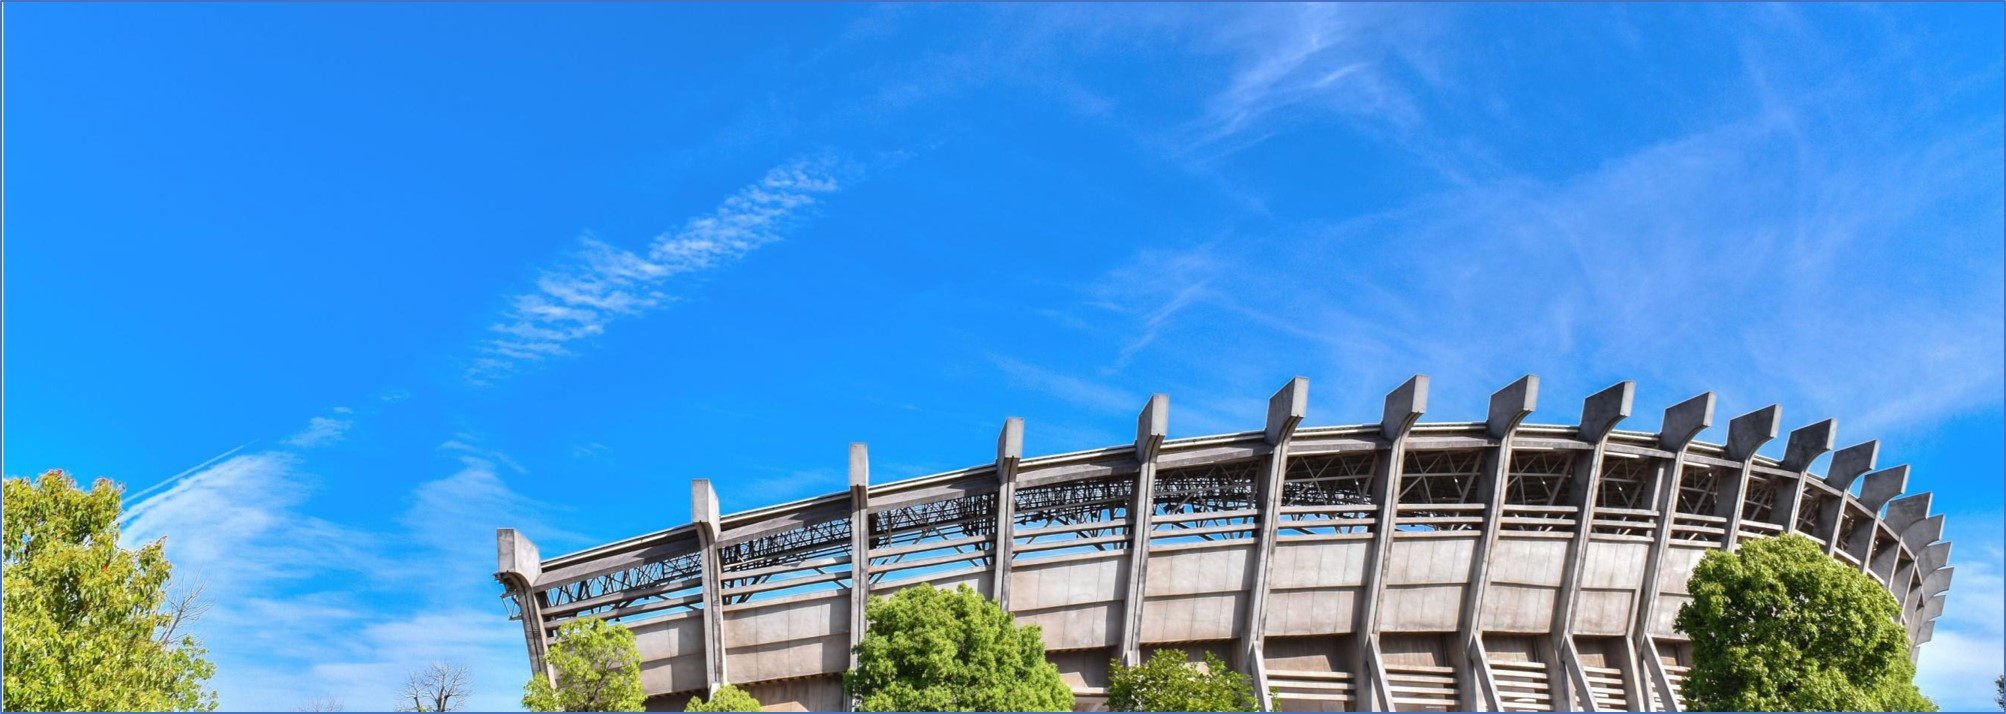
\includegraphics[width=0.8\linewidth]{figures/csu}
	\caption{中南大学}
	\label{fig:csu}%标签,以备交叉引用
\end{figure}

如表\ref{tab:scores}所示,
%三线表,toprule和bottom分别是顶线和底线,midrule是中间的线
%\topcaption是我重新定义的表题命令,目的是减小表题与表格间距离,见dissertation.tex文件105-110行
\begin{table}[H]
\centering
\topcaption{成绩单}\label{tab:scores}
\begin{tabular}{ccc}
	\toprule 
	姓名 & 高等数学 & 线性代数 \\
	\midrule
	张三 & 100 & 100 \\
	李四 & 101 & 101 \\
	\bottomrule
\end{tabular}
\end{table}
